% =====================================================================
%  Introduction to Deep Learning — Class 3
%  Topic: Perceptrons and the Perceptron Learning Algorithm
%
%  Plots are produced by  src/make_figures.py  (SciencePlots "science"
%  preset, Fira Sans).  Concepts follow Rojas (1996), Ch. 3-4.
%
%  Compile:  xelatex main.tex   (run twice)
% =====================================================================
\documentclass[aspectratio=169, 11pt]{beamer}

\usetheme{metropoliscustom}

\usepackage{graphicx}
\DeclareGraphicsExtensions{.pdf,.png,.jpg}  % prefer vector PDF
\graphicspath{{figs/}{Class03_Perceptrons_PLA/B_Recreated_Figures/figs/}}
\usepackage{amsmath, amssymb}
\usepackage{bm}
\usepackage{tikz}
\usetikzlibrary{arrows.meta, positioning, calc, decorations.pathreplacing,
                backgrounds, fit}
\tcbuselibrary{skins}

% ---- shared palette -------------------------------------------------
\definecolor{shc}{HTML}{341651}    % M-P side / class N
\definecolor{tealc}{HTML}{1C7293}  % activations / boundary
\definecolor{dpc}{HTML}{800000}    % perceptron side / class P
\definecolor{accc}{HTML}{B8860B}   % fourth series

% ---- parallel strip: McCulloch-Pitts (left) vs Perceptron (right)
\newcommand{\mppar}[2]{%
  \vfill
  {\footnotesize
  \begin{tcolorbox}[enhanced, sidebyside, sidebyside align=top,
                    lefthand ratio=0.485,
                    segmentation style={shc!35, line width=0.6pt},
                    colback=shc!5, colframe=shc!35, boxrule=0.5pt,
                    arc=1.5mm, left=2mm, right=2mm, top=0.8mm, bottom=0.8mm]
    {\color{shc}\textbf{M--P}}\;\; #1
  \tcblower
    {\color{dpc}\textbf{PERCEPTRON}}\;\; #2
  \end{tcolorbox}}%
  \vspace{0.6em}%
}

\newcommand{\figsource}[1]{{\scriptsize\color{mcMuted} #1}}

% ---- a unit drawn as a circle with its activation inside ------------
\newcommand{\unit}[4]{%
  \node[circle, draw=#3, fill=#3!6, line width=1.0pt,
        minimum size=16mm, inner sep=0pt] (#1) at #2 {};
  \begin{scope}
    \clip #2 circle (0.8);
    \draw[tealc, line width=1.6pt]
      ($#2+(-0.80,-0.42)$) -- ($#2+(0.03,-0.42)$) -- ($#2+(0.74,0.45)$);
  \end{scope}
  \node[font=\large, #3] at ($#2+(0,1.12)$) {#4};
}
\newcommand{\plainunit}[4]{%
  \node[circle, draw=#3, fill=black!4, line width=1.0pt,
        minimum size=16mm, inner sep=0pt, font=\normalsize]
        (#1) at #2 {#4};
}

% =====================================================================
\title{Perceptrons and the Perceptron Learning Algorithm}
\subtitle{Weighted threshold units, and how they learn}
\author{Introduction to Deep Learning \ \textperiodcentered\ Class 3}
\institute{}
\date{29 July}

\footleft{DA3409 Deep Learning}
\footright{Perceptrons and the PLA}
\titlelogos{}

\begin{document}

\maketitle

\begin{frame}{Outline}
  \tableofcontents
\end{frame}

% =====================================================================
\section{From Threshold Logic to the Perceptron}
% =====================================================================

\begin{frame}{Recap: Last Class}
  \begin{itemize}
    \item A McCulloch--Pitts unit fires when
          $x_1+\cdots+x_n \ge \theta$ --- inputs are summed
          with \alert{equal weight}
    \item Geometrically it is a \alert{separating plane}, but
          the planes are always \alert{parallel}: only the
          offset changes
    \item Almost every Boolean function is out of reach ---
          by $n=5$ barely $0.002\%$ are linearly separable
  \end{itemize}
  \vspace{0.3em}
  \begin{redhighlight}
    Give each input its own \alert{weight} and add a
    \alert{bias}: the plane can now take any orientation and
    offset. This is the \alert{perceptron}.
  \end{redhighlight}
\end{frame}

\begin{frame}{A little history: Rosenblatt's perceptron}
  \centering
  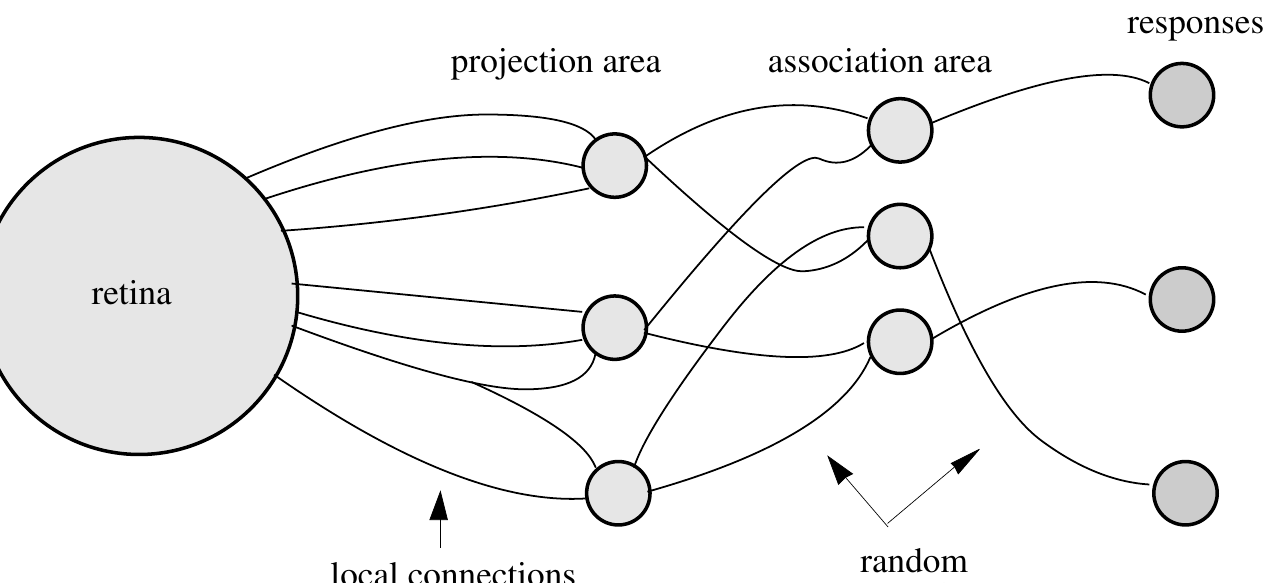
\includegraphics[height=0.33\textheight]{classic_perceptron}
  \\[0.1em]
  \figsource{Rojas (1996), Fig.~3.1: the classical perceptron
  [after Rosenblatt 1958].}
  \vspace{0.2em}
  \begin{itemize}\setlength{\itemsep}{0pt}
    \item Rosenblatt (1958) wired a \alert{retina} of pixels to
          weighted threshold units --- built to \alert{learn} to
          recognise patterns
    \item Its only formal difference from a McCulloch--Pitts
          unit is the presence of \alert{weights}
         % \hfill{\scriptsize Rojas (1996), \S3.1}
   % \item It drew great excitement --- and, later, a famous
   %       controversy over its limits
  \end{itemize}
\end{frame}

\begin{frame}{The perceptron: a weighted threshold unit}
  \begin{columns}[T, onlytextwidth]
    \begin{column}{0.52\textwidth}
      \centering
      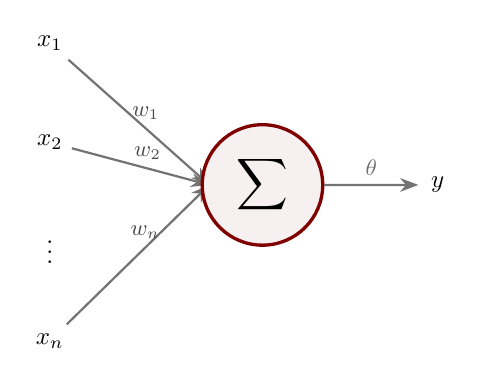
\begin{tikzpicture}[>=Stealth, line width=0.8pt,
          scale=0.90, transform shape, font=\normalsize]
        \foreach \i/\y in {1/2.1, 2/0.7, n/-2.1}{
          \node (x\i) at (0,\y) {$x_{\i}$};
          \draw[->, black!55] (x\i) -- node[above, pos=0.55,
            font=\small, black!70] {$w_{\i}$} (2.25,0.1);
        }
        \node at (0,-0.75) {$\vdots$};
        \node[circle, draw=dpc, fill=dpc!6, line width=1.2pt,
              minimum size=17mm, inner sep=0pt] (u) at (3.0,0.1)
              {\Large$\displaystyle\sum$};
        \draw[->, black!55] (u) -- node[above, font=\small]
              {$\theta$} (5.2,0.1);
        \node[right, font=\normalsize] at (5.25,0.1) {$y$};
      \end{tikzpicture}
    \end{column}
    \hfill
    \begin{column}{0.44\textwidth}
      \vspace{0.5em}
      \[
        y=\begin{cases}
          1 & \text{if } \sum_i w_i x_i \ge \theta\\[2pt]
          0 & \text{otherwise}
        \end{cases}
      \]
      \begin{itemize}\setlength{\itemsep}{2pt}
        \item Each input carries a real \alert{weight} $w_i$
        \item Rosenblatt (1958); weights make the plane
              \alert{freely orientable}
      \end{itemize}
    \end{column}
  \end{columns}
  \mppar{fixed unit weights}{\alert{learnable} real weights}
\end{frame}

\begin{frame}{Weights tilt the separating line}
  \begin{columns}[T, onlytextwidth]
    \begin{column}{0.52\textwidth}
      \centering
      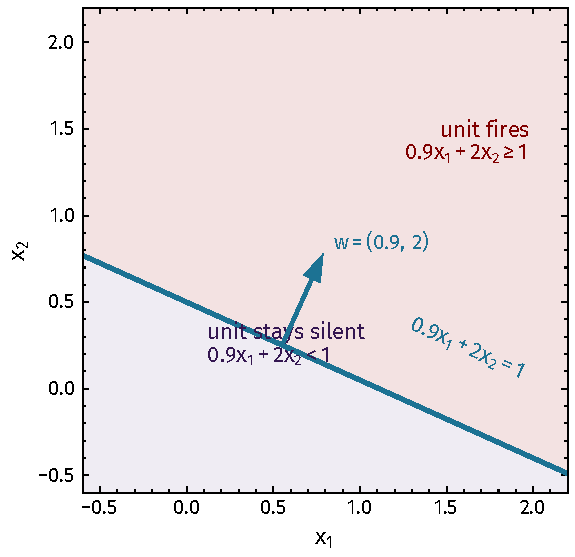
\includegraphics[height=0.50\textheight]{regions}
    \end{column}
    \hfill
    \begin{column}{0.44\textwidth}
      \vspace{0.4em}
      {\small A perceptron with weights $(0.9,\,2)$ and
      threshold $1$ tests}
   $$     0.9\,x_1 + 2\,x_2 \;\ge\; 1 $$\vspace{-1cm}
      \begin{itemize}\setlength{\itemsep}{1pt}
        \item The equality is the \alert{boundary}; the two
              inequalities name the two \alert{regions}
        \item $\mathbf{w}$ is \alert{normal} to the line and
              points into the firing region
        \item The slope is now \alert{arbitrary}
      \end{itemize}
    \end{column}
  \end{columns}
\end{frame}

\begin{frame}{What the weights and the bias each control}
  \centering
  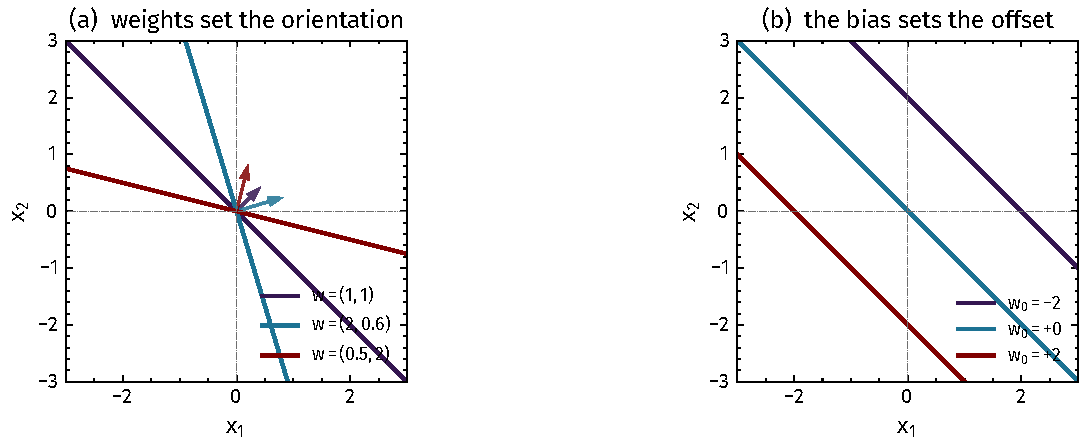
\includegraphics[height=0.42\textheight]{weights_bias}
  \\[0.15em]
  \figsource{(a) three weight vectors with the same bias: the
  boundary $\mathbf{w}\!\cdot\!\mathbf{x}=0$ takes a different
  \emph{orientation} in each case (arrows show $\mathbf{w}$,
  always normal to its line).
  (b) one weight vector with three biases: the boundary keeps
  its orientation and simply \emph{shifts}.}
  \mppar{parallel planes only}{any orientation and offset}
\end{frame}

\begin{frame}{The bias trick}
  \centering
  \begin{tikzpicture}[>=Stealth, line width=0.9pt,
      scale=0.46, transform shape, font=\normalsize]
    % --- left: explicit threshold
    \foreach \i/\y in {1/1.5, 2/0.0, 3/-1.5}{
      \node (a\i) at (0,\y) {$x_{\i}$};
      \draw[->, black!55] (a\i) -- (2.0,0.0);
    }
    \node[circle, draw=dpc, fill=dpc!6, line width=1.2pt,
          minimum size=16mm, inner sep=0pt] (ga) at (2.8,0.0)
          {\large$\theta$};
    \draw[->, black!55] (ga) -- (4.4,0.0);
    % --- the equivalence arrow
    \node[font=\Large, mcMuted] at (5.3,0.0) {$\Longleftrightarrow$};
    % --- right: threshold folded in as a weight from a constant 1
    \foreach \i/\y in {1/1.5, 2/0.0, 3/-1.5}{
      \node (b\i) at (6.6,\y) {$x_{\i}$};
      \draw[->, black!55] (b\i) -- (8.6,0.0);
    }
    \node[shc] (one) at (6.6,-2.9) {$1$};
    \draw[->, shc, line width=1.1pt] (one) --
      node[below, pos=0.55, font=\small, shc] {$-\theta$} (8.6,0.0);
    \node[circle, draw=dpc, fill=dpc!6, line width=1.2pt,
          minimum size=16mm, inner sep=0pt] (gb) at (9.4,0.0)
          {\large$0$};
    \draw[->, black!55] (gb) -- (11.0,0.0);
  \end{tikzpicture}
  \vspace{0.1em}
  {\small Both units compute the same function:}
  \vspace{-0.3em}
  \[
    \textstyle\sum_i w_i x_i \ge \theta
    \quad\Longleftrightarrow\quad
    \textstyle\sum_i w_i x_i + (-\theta)\cdot 1 \ge 0 .
  \]
  \vspace{-0.7em}
  \begin{itemize}\setlength{\itemsep}{0pt}
    \item An input clamped to $1$ with weight $-\theta$; the
          unit now compares against \alert{zero}
    \item That weight is the \alert{bias} --- \alert{learned
          like any other}, so one rule updates weights and
          threshold together
        %  \hfill{\scriptsize Rojas (1996), \S3.1.1}
  \end{itemize}
  \mppar{threshold $\theta$ fixed by the designer}
        {threshold becomes a \alert{learnable} bias weight}
\end{frame}

\begin{frame}{Extended input space}
  With the bias folded in, every input becomes an
  \alert{extended vector} and the test is homogeneous:
  \[
    \tilde{\mathbf{x}} = (x_0,\,x_1,\dots,x_n),
    \qquad
    \tilde{\mathbf{w}} = (-\theta,\,w_1,\dots,w_n),
    \qquad
    \tilde{\mathbf{w}}\cdot\tilde{\mathbf{x}} \ge 0.
  \]
  \begin{itemize}\setlength{\itemsep}{0pt}
    \item One vector holds everything --- no separate threshold
    \item The separating plane now passes through the
          \alert{origin} of $(n{+}1)$-space
    \item Data split into $P$ (target $1$) and $N$ (target $0$);
          seek $\mathbf{w}$ with
          $\tilde{\mathbf{w}}\!\cdot\!\tilde{\mathbf{x}}>0$ on $P$, $<0$ on $N$
         % \hfill{\scriptsize Rojas (1996), \S4.1.2}
  \end{itemize}
  \mppar{hand-designed weights}
        {weights to be \alert{found} from labelled data}
\end{frame}

% =====================================================================
\section{The Learning Problem}
% =====================================================================

\begin{frame}{What does it mean to `learn'?}
  \centering
  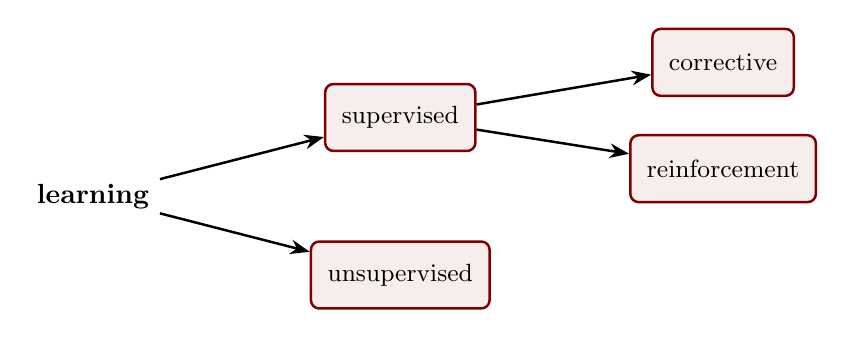
\begin{tikzpicture}[>=Stealth, line width=0.9pt,
      lvl/.style={font=\normalsize},
      leaf/.style={rounded corners=3pt, draw=dpc, fill=dpc!7,
                   font=\small, inner xsep=6pt, minimum height=0.85cm}]
    \node[lvl] (root) at (0,0) {\textbf{learning}};
    \node[leaf] (sup) at (3.9,1.0) {supervised};
    \node[leaf] (uns) at (3.9,-1.0) {unsupervised};
    \node[leaf] (cor) at (8.0,1.7) {corrective};
    \node[leaf] (rei) at (8.0,0.35) {reinforcement};
    \draw[->] (root)--(sup); \draw[->] (root)--(uns);
    \draw[->] (sup)--(cor); \draw[->] (sup)--(rei);
  \end{tikzpicture}
  \vspace{0.5em}
  \begin{itemize}\setlength{\itemsep}{1pt}
    \item \alert{Supervised}: each input comes with a target;
          \alert{unsupervised}: the network finds structure on
          its own
    \item Supervised splits into \alert{corrective} (fix the
          error directly) and \alert{reinforcement}
    \item The \alert{perceptron} rule is supervised with error
          correction
        %  \hfill{\scriptsize Rojas (1996), \S4.1.1}
  \end{itemize}
\end{frame}

\begin{frame}{Two dual viewpoints}
  \centering
  
\includegraphics[height=0.38\textheight]{duality}
  \\[0.1em]
  \figsource{$\mathbf{w}\!\cdot\!\mathbf{x}=0$ is symmetric in
  $\mathbf{w}$ and $\mathbf{x}$. (a) fix $\mathbf{w}$ and the
  \emph{inputs} split into half-planes. (b) fix one input
  $\mathbf{x}$ and the \emph{weights} split the same way ---
  $\mathbf{x}$ becomes the normal, each candidate $\mathbf{w}$
  a point.}
  \vspace{0.05em}
  \begin{redhighlight}
    Learning is a search in \alert{weight space} for a point on
    the correct side of every data plane.
  \end{redhighlight}
\end{frame}

\begin{frame}{Learning as a search in weight space}
  \begin{itemize}\setlength{\itemsep}{2pt}
    \item A network is a \alert{parametric system}: fix the
          architecture, and the weights are free parameters
    \item ``Learning'' means \alert{searching} weight space
          for values that classify the training data correctly
    \item Every input vector $\mathbf{x}$ imposes one
          constraint --- it carves weight space into the
          weights that get it right and those that do not
    \item The solutions form the \alert{intersection} of all
          those half-spaces
  \end{itemize}
  \mppar{weights fixed by the designer}
        {weights \alert{searched} to fit the data}
\end{frame}

\begin{frame}{The error surface}
  \centering
  
\includegraphics[height=0.40\textheight]{error_surface}
  \\[0.1em]
  \figsource{A perceptron with fixed threshold $\theta=1$
  learning \textbf{AND}; the error is the number of the four
  patterns it gets wrong, as $(w_1,w_2)$ vary.
  (a) the surface as a landscape --- flat terraces with sharp
  steps, since the error is a count.
  (b) the same surface from above; the white outline bounds the
  triangular \alert{solution region} where the error is zero.
  (c) the path the algorithm takes across it.}
  \vspace{0.1em}
  {\small The three panels are the \emph{same} surface: a
  landscape, a map, and a route across it.
%  \hfill{\scriptsize after Rojas (1996), Fig.~4.5}
}
\end{frame}

\begin{frame}{Absolute linear separability}
  \begin{redhighlight}
   Two sets $P$ and $N$ of points in an $n$-dimensional space are
called absolutely linearly separable if $(n + 1)$ real numbers $w_1,\ldots, w_{n+1}$ exist such that every point $(x_1, x_2,\ldots , x_n)\in  P$ satisfies $\sum\limits_{i=1}^n w_ix_i > w_{n+1}$ and  every point $(x_1, x_2,\ldots , x_n)\in  N$  satisfies $\sum\limits_{i=1}^n w_ix_i < w_{n+1}$.
  \end{redhighlight}
  \begin{itemize}\setlength{\itemsep}{2pt}
%    \item The PLA needs a \alert{strict} separation: every
          % point of $P$ on the \emph{open} positive side, every
          % point of $N$ on the open negative side
    \item If a separating plane exists, one can always be
          found with a \alert{margin} -- no data point lying
          exactly on it
 %   \item This \alert{absolute} separability is what makes the
        %  convergence proof work
  \end{itemize}
  \vspace{0.3em}
  \begin{redhighlight}
    ``Separable'' is not quite enough --- we need a little room
    on each side. Then learning is guaranteed to finish.
  \end{redhighlight}
\end{frame}

% =====================================================================
%\section{The Perceptron Learning Algorithm}
% =====================================================================

\begin{frame}{Learning as error correction}
  \centering
  \begin{tikzpicture}[>=Stealth, line width=0.9pt, scale=0.68,
      transform shape,
      b/.style={rounded corners=3pt, draw=dpc, fill=dpc!7,
                align=center, minimum height=0.95cm,
                inner xsep=6pt, font=\small},
      lbl/.style={font=\scriptsize, mcMuted}]
    \node[b] (p) {present\\a pattern};
    \node[b, right=9mm of p] (c) {classified\\correctly?};
    \node[b, right=11mm of c] (u) {update:\\$w \pm x$};
    \node[b, below=8mm of c] (d) {done};
    \draw[->] (p)--(c);
    \draw[->] (c)-- node[above, lbl] {no} (u);
    \draw[->] (u) -- ++(0,1.15) -| (p);
    \draw[->] (c)-- node[right, lbl] {all correct} (d);
    \draw[->] (c.north) ++(0,0) .. controls +(0,0.9) and +(0,0.9) ..
      node[above, lbl] {yes} (p.north);
  \end{tikzpicture}
  \vspace{0.4em}
  \begin{itemize}\setlength{\itemsep}{1pt}
    \item Start from a \alert{random} weight vector; present
          training examples one at a time
    \item Classified \alert{correctly} $\to$ change nothing
    \item \alert{Wrong} $\to$ nudge the weights toward the right
          decision, then carry on
    \item Each step uses \alert{one example} and the
          \alert{current} weights only --- local, online, and
          strikingly simple
  \end{itemize}
\end{frame}

\begin{frame}{The algorithm}
  Sets $P$ and $N$ of extended vectors. Seek $\mathbf{w}$ with
  $\mathbf{w}\!\cdot\!\mathbf{x}>0$ on $P$ and
  $\mathbf{w}\!\cdot\!\mathbf{x}\le 0$ on $N$
%  (Rojas, 1996, \S4.2):
  \vspace{0.2em}
  \begin{tcolorbox}[colback=dpc!4, colframe=dpc!40,
                    boxrule=0.5pt, arc=1mm, left=3mm]
  {\small
  \textbf{start:} random $\mathbf{w}_0$, \; $t:=0$\\[2pt]
  \textbf{test:} pick $\mathbf{x}\in P\cup N$ at random\\
  \quad if correctly classified: go to \textbf{test}\\
  \quad if $\mathbf{x}\in P$ and
        $\mathbf{w}_t\!\cdot\!\mathbf{x}\le 0$:
        go to \textbf{add}\\
  \quad if $\mathbf{x}\in N$ and
        $\mathbf{w}_t\!\cdot\!\mathbf{x}\ge 0$:
        go to \textbf{subtract}\\[2pt]
  \textbf{add:} $\mathbf{w}_{t+1}=\mathbf{w}_t+\mathbf{x}$,
        \ $t{:=}t{+}1$; go to \textbf{test}\\[2pt]
  \textbf{subtract:} $\mathbf{w}_{t+1}=\mathbf{w}_t-\mathbf{x}$,
        \ $t{:=}t{+}1$; go to \textbf{test}}
  \end{tcolorbox}
\end{frame}

\begin{frame}{Why the update works}
  \centering
  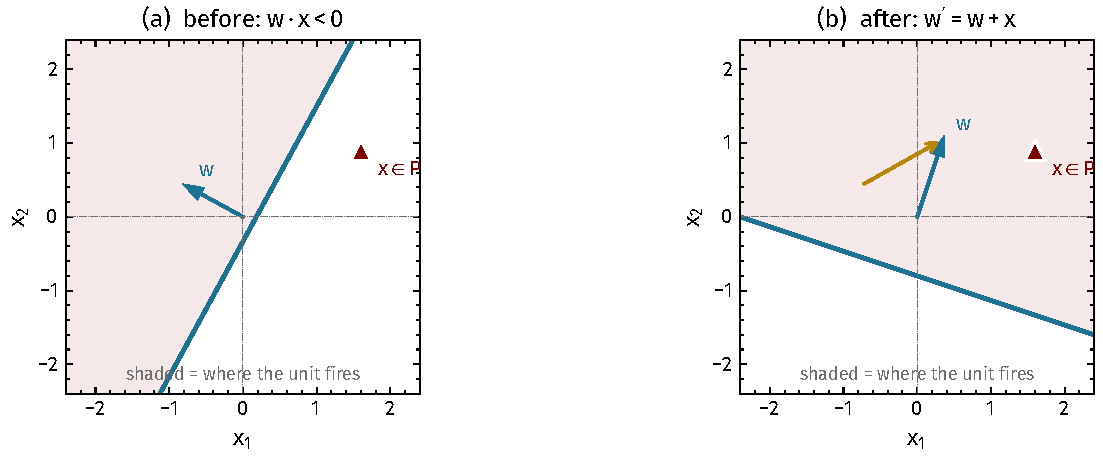
\includegraphics[height=0.40\textheight]{update_step}
  \\[0.1em]
  \figsource{A point $\mathbf{x}\in P$ the current $\mathbf{w}$
  gets wrong: it lies outside the shaded firing half-plane.
  (a) before, $\mathbf{w}\!\cdot\!\mathbf{x}<0$.
  (b) after $\mathbf{w}'=\mathbf{w}+\mathbf{x}$, the weight has
  rotated toward $\mathbf{x}$ (amber arrow) and the half-plane
  now covers it.}
  \vspace{0.05em}
  {\small $\mathbf{w}'\!\cdot\!\mathbf{x}
   = \mathbf{w}\!\cdot\!\mathbf{x} + \lVert\mathbf{x}\rVert^2$
  --- the dot product \alert{always increases}.}
\end{frame}

\begin{frame}{The algorithm running}
  \centering
  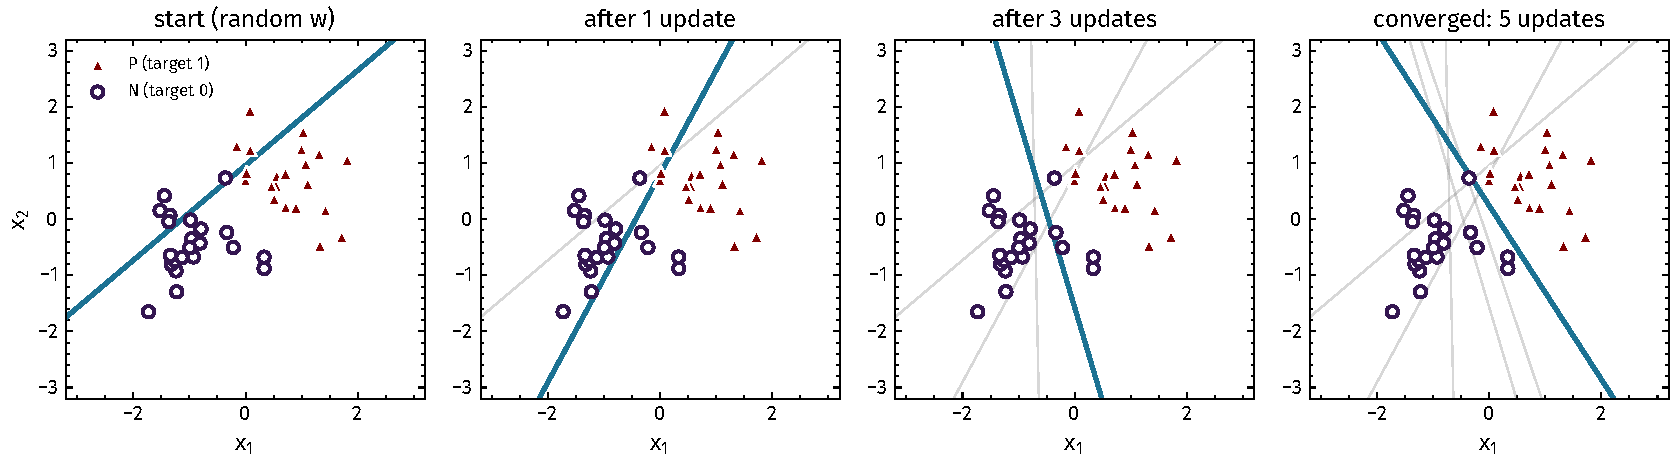
\includegraphics[height=0.40\textheight]{pla_run}
  \\[0.15em]
  \figsource{Two separable clouds, $P$ (triangles) and $N$
  (circles). The teal line is the current decision boundary;
  faint grey lines are the boundaries it held earlier. Each
  panel is a later moment in the same run --- the boundary
  swings across the data and stops as soon as every point is
  on its correct side.}
  \mppar{no update rule --- weights set by hand}
        {each mistake rotates $\mathbf{w}$ the right way}
\end{frame}

\begin{frame}{The update, seen in weight space}
  \centering
  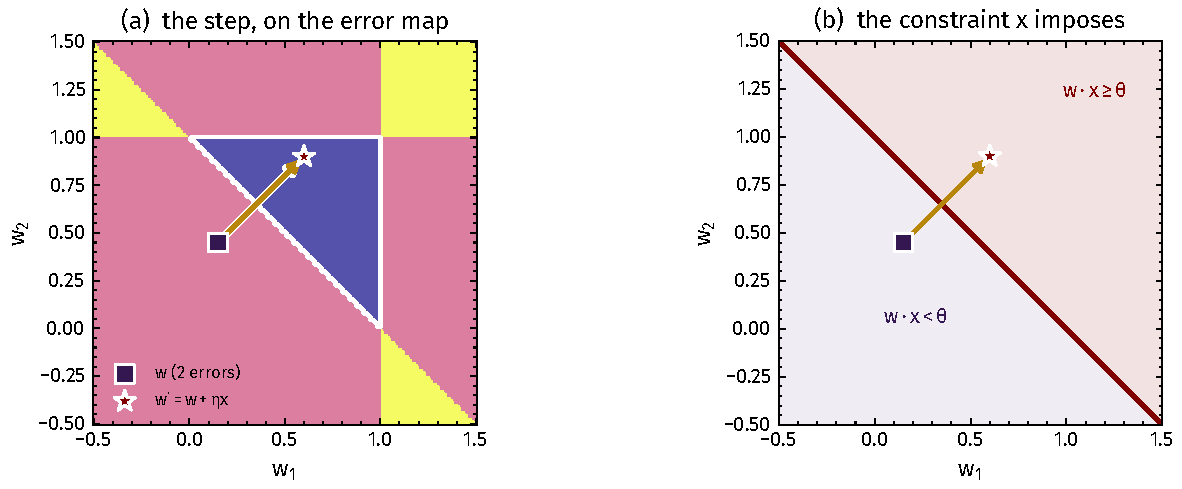
\includegraphics[height=0.44\textheight]{update_ws}
  \\[0.1em]
  \figsource{The same AND problem as before.
  (a) one correction moves $\mathbf{w}$ (square) to
  $\mathbf{w}'$ (star) --- straight off a high-error terrace
  and into the solution region.
  (b) the same step against the constraint that the offending
  pattern $\mathbf{x}$ imposes: it demands
  $\mathbf{w}\!\cdot\!\mathbf{x}\ge\theta$, and the update
  carries $\mathbf{w}$ across that line.}
  \vspace{0.1em}
  {\small Each pattern contributes one such constraint; a
  solution satisfies them all at once.
 % \hfill{\scriptsize after Rojas (1996), Fig.~4.11}
 }
\end{frame}

\begin{frame}{Fixing the error in one step}
  The plain rule nudges; we can instead \alert{fully correct}
  a mistake. For $\mathbf{x}\in P$ with
  $\mathbf{w}\!\cdot\!\mathbf{x} = -\delta \le 0$, set
  %(Rojas, 1996, \S4.2.3):
  \[
    \mathbf{w}' = \mathbf{w}
    + \frac{\delta + \varepsilon}{\lVert\mathbf{x}\rVert^2}\,
    \mathbf{x}
    \quad\Longrightarrow\quad
    \mathbf{w}'\!\cdot\!\mathbf{x} = \varepsilon > 0.
  \]
  \begin{itemize}\setlength{\itemsep}{1pt}
    \item One update moves $\mathbf{x}$ just past the boundary,
          by a margin $\varepsilon$
    \item Small $\varepsilon$ avoids overshooting into a worse
          region
    \item This \alert{corrective} variant learns faster than
          plain add/subtract
  \end{itemize}
  \mppar{no notion of correction}
        {each step \alert{eliminates} one error outright}
\end{frame}

% =====================================================================
\section{Convergence and Limits}
% =====================================================================

\begin{frame}{The perceptron convergence theorem}
  \begin{redhighlight}
    If $P$ and $N$ are \alert{linearly separable}, the
    perceptron learning algorithm makes only a \alert{finite}
    number of weight updates --- it reaches a separating
    $\mathbf{w}$ in finite time.
    
  \end{redhighlight}
  \vspace{0.4em}
  \begin{itemize}\setlength{\itemsep}{2pt}
    \item Idea of the proof: if a solution $\mathbf{w}^{*}$
          exists, every update increases the alignment
          $\mathbf{w}\!\cdot\!\mathbf{w}^{*}$ faster than it
          grows $\lVert\mathbf{w}\rVert$
    \item Bounding those two quantities forces the number of
          updates to be finite
    %      \hfill{\scriptsize Rojas (1996), \S4.2--4.3}
    \item A guarantee of \alert{termination}, not of speed
  \end{itemize}
\end{frame}

% \begin{frame}{How long can it take?}
%   \centering
%   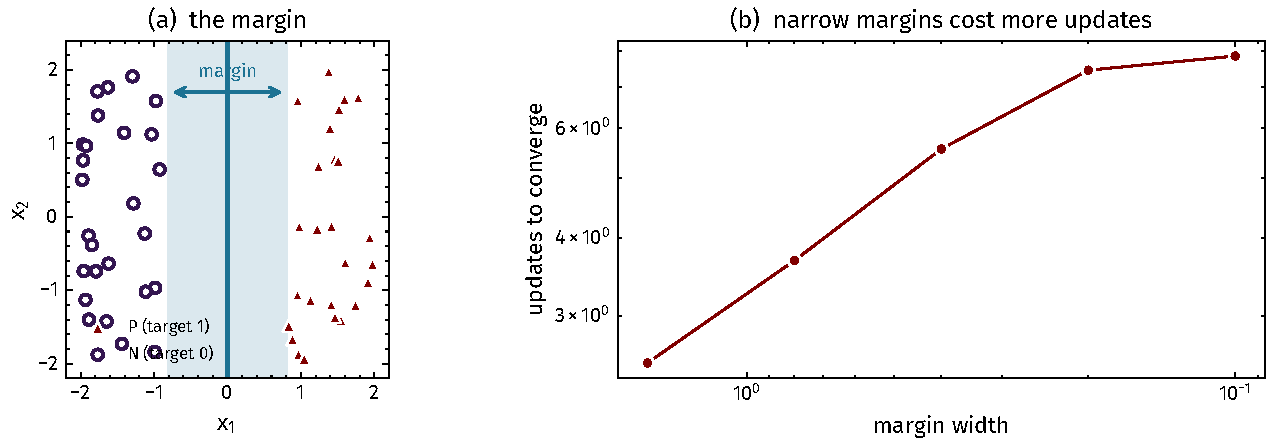
\includegraphics[height=0.38\textheight]{margin}
%   \\[0.1em]
%   \figsource{(a) the \emph{margin} is the empty corridor
%   between the classes. (b) average updates as that corridor
%   narrows (log--log, margin shrinking to the right): the cost
%   climbs with the inverse squared margin.}
%   \mppar{no learning --- nothing to time}
%         {finite, but slow when the margin is thin}
% \end{frame}


\begin{frame}{The limit: XOR and non-separable data}
  \begin{columns}[T, onlytextwidth]
    \begin{column}{0.44\textwidth}
      \centering
      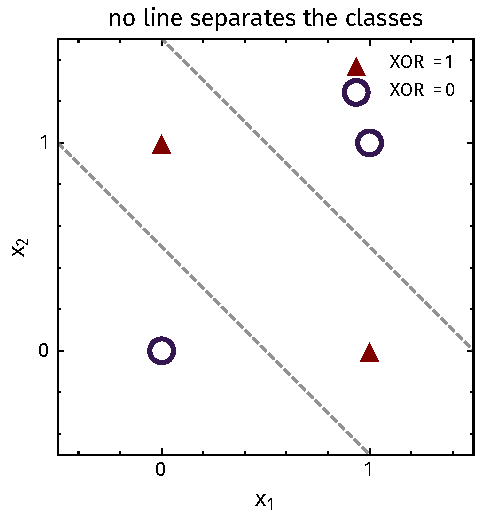
\includegraphics[height=0.42\textheight]{xor}
    \end{column}
    \hfill
    \begin{column}{0.52\textwidth}
      \vspace{0.4em}
      \begin{itemize}\setlength{\itemsep}{2pt}
        \item A single perceptron computes exactly the
              \alert{linearly separable} functions --- any
              orientation, but still one line
        \item \alert{XOR} is not separable, so the PLA
              \alert{never terminates} on it
        \item On non-separable data the \alert{pocket
              algorithm} keeps the best weights seen so far
              %\hfill{\scriptsize Rojas, \S4.2.4}
      \end{itemize}
    \end{column}
  \end{columns}
  \begin{redhighlight}
    One layer is still a linear classifier. XOR needs a
    \alert{hidden layer} --- the shallow network.
  \end{redhighlight}
\end{frame}

\begin{frame}{Takeaways}
  \begin{enumerate}\setlength{\itemsep}{2pt}
    \item A \alert{perceptron} is a threshold unit with
          \alert{learnable weights} and a \alert{bias} --- its
          boundary is a freely oriented hyperplane
    \item The bias trick makes the test homogeneous:
          $\tilde{\mathbf{w}}\!\cdot\!\tilde{\mathbf{x}}\ge 0$
    \item The \alert{PLA} corrects only on mistakes: add
          $\mathbf{x}$ for a missed positive, subtract for a
          missed negative
    \item It \alert{provably converges} on separable data ---
          but slowly when the margin is thin, and never on
          XOR
  \end{enumerate}
  \vspace{0.3em}
  \begin{redhighlight}
    Class~5: stack weighted units into layers --- the shallow
    neural network.
  \end{redhighlight}
\end{frame}

\begin{frame}{References}
  \footnotesize
  \begin{itemize}\setlength{\itemsep}{3pt}
    \item R.~Rojas. \textit{Neural Networks: A Systematic
          Introduction.} Springer, 1996. Chapters 3--4 ---
          weighted networks, input/weight-space duality,
          the learning algorithm and its convergence.
    \item F.~Rosenblatt (1958). ``The perceptron: a
          probabilistic model for information storage and
          organization in the brain.'' \textit{Psychological
          Review}, 65(6), 386--408.
    \item Plots generated with \texttt{src/make\_figures.py}
          (NumPy, Matplotlib, SciencePlots).
  \end{itemize}
\end{frame}

\begin{frame}[standout]
  Questions?
\end{frame}

\end{document}
